% 3. Protokoll

\chapter{Messprotokoll}
\label{chap:protokoll}
Zu jeder dat-File wird auch eine bmp-File des Fourierspektrums abgespeichert mit selben Dateinamen.
\section*{Mittelung der Fouriertransformation}
Dateibeginn: \textit{Zeit\_Datum\_G11\_averaging\_}
\paragraph{a)}\textbf{Fourierentwicklung Sinus, Rechteck und Dreieck}\\
Dateinamen:\\
\textit{41a\_Sinus\_A1V\_F1kHz\_n10.dat}\\
\textit{41a\_Dreieck\_A1V\_F1kHz\_n10.dat}\\
\textit{41a\_Rechteck\_A1V\_F1kHz\_n10.dat}

A, F, n = Amplitude, Eingestellte Frequenz (später f), Anzahl der Mittelungen

\paragraph{b)}\textbf{Fourierspektrum Sinus-Signal}\\
Dateinamen:\\
\textit{41b\_Sinus\_A1V\_F1kHz\_n100.dat}

\paragraph{c)}\textbf{Mittelung und Rauschen}\\
Dateinamen:\\ 
\textit{41c\_Rechteck\_A1V\_F1kHz\_nX\_Rau\_BW20MHz\_AMD120pc.dat}\\
$X$ = 0, 10, 50, 100

Rau, BW, AMD = mit Rauschen, Bandbreite, AM Depth (pc = \%)

\paragraph{d)+e)}\textbf{Oberwellen-Abstand + Bandbreite des Rauschens}\\
Dateinamen:\\
\textit{41d\_Rechteck\_A1V\_F1kHz\_n0\_Rau\_BW20MHz\_AMDN.dat} \\$N$ = 120pc, 100pc, 50pc, 10pc

\textit{41d\_Rechteck\_A1V\_F1kHz\_n0\_Rau\_BWN\_AMD100pc.dat} \\$N$ = 20MHz, 10MHz, 5MHz, 100kHz, 10kHz, 1kHz
\newpage
\section*{Abtasttheorem}
Dateibeginn: \textit{Zeit\_Datum\_G11\_sampling\_}
\paragraph{a)}\textbf{Variation Abtastrate + Frequenz}\\
Dateinamen:\\
\textit{42a\_Sinus\_f20kHz\_A1V\_fsN.dat}\tab $N$ = 1kHz bis 100khz\\
\textit{42a\_Sinus\_fN\_A1V\_fs20khz.dat}\tab $N$ = 1kHz bis 50kHz

\paragraph{b)}\textbf{Fourierspektrum bei verschiedenen Abtastraten}\\
Dateinamen:\\
\textit{42b\_Dreieck\_f3kHz\_A1V\_fsN.dat}\tab $N$ = 6kHz bis 9kHz

\section*{Signalfilterung}
Dateibeginn: \textit{Zeit\_Datum\_G11\_filtering\_}
\paragraph{a)}\textbf{Frequenzgang von Tiefpassfilter}\\
Dateinamen:\\
\textit{43a\_Sinus\_f100Hz\_A1V\_Rau\_BW20MHz\_AMD120pc\_Fil\_X\_Lopa\_OrN\_Uf1k.dat}\\
$X$ = Bu (Butterworth), Ch (Chebyshev), InCh (Chebyshev$^{-1}$), El (Elliptic), Be (Bessel)\\
$N$ = 1, 2, 5, 10 (Ordnung des Filters)

Lopa, Hipa, Bapa, Fil, Or = Lowpass, Highpass, Bandpass, Filter, Ordnung\\
Lf, Uf = Lower Frequency, Upper Frequnecy (1k bedeutet 1kHz)

\paragraph{b)}\textbf{Sprungantwort}\\
Dateinamen:\\
\textit{43b\_Rechteck\_f100Hz\_A1V\_Fil\_X\_Y\_OrN\_Uf1k.dat}\\
$X$, $Y$, $N$ = (Bu, Ch, InCh, El, Be); (Lopa, Hipa); (1, 2, 5, 10)
\newpage
\paragraph{c)}\textbf{Vergleich Analog zu Digital}
Filterbeschreibung: Ithaco 4302
\begin{center}
    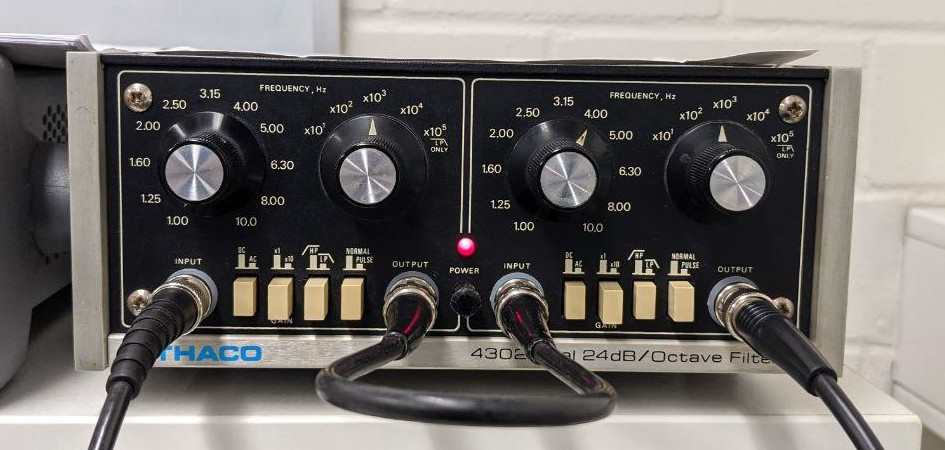
\includegraphics[scale = 0.4]{EinstellungAnalogFilter.jpg}
    \captionof{figure}{Einstellungen des Analogfilters als Bandpass}
    \label{image:analogFilter}
\end{center}
Dateinamen:\\
\textit{43c\_Sinus\_f2kHz\_A1V\_AnalFil\_Bu\_Bapa\_Or1\_Lf1kHz\_Uf4kHz.dat}\\
\textit{43c\_Sinus\_f2kHz\_A1V\_DigiFil\_Bu\_Bapa\_Or1\_Lf1kHz\_Uf4kHz.dat}\\
\textit{43c\_Rechteck\_f2kHz\_A1V\_AnalFil\_Bu\_Bapa\_Or1\_Lf1kHz\_Uf4kHz.dat}\\
\textit{43c\_Rechteck\_f2kHz\_A1V\_DigiFil\_Bu\_Bapa\_Or1\_Lf1kHz\_Uf4kHz.dat}

AnalFil, DigiFil = Analog Filter, Digital Filter

\paragraph{d)}\textbf{Verbesserung mit Bandpass 4.Ordnung}\\
Formel für Spannungsverhältnis in dB:
\begin{gather}
    L = 20 \log_{10}\left(\frac{U}{U_0}\right)
\end{gather}
Daraus folgt für ein Signal-Rausch-Verhältnis von $L=$10dB: $\frac{U}{U_0} = 3,16$\\
$\Rightarrow$ AMD $\approx$ 70\% (Eingestellt nach Gefühl am Oszilloskop). Bester Kompromiss bei einer Lower Frequency von 10mHz und einer Upper Frequency von 55kHz.\\
Dateinamen:\\
\textit{43d\_Rechteck\_f1kHz\_A1V\_Rau\_BW20MHz\_AMD70pc\_DigiFil\_Bu\_Bapa\_Or4\\
\_Lf10mHz\_Uf55kHz}
\newpage
\section*{Lock-In Technik}
Modell Lock-In: SR830 DSP
Messfehler Lock-In:
\begin{itemize}
    \item Amplitude = 0,0001 (V, mV, $\mu$V, nV, pV) (Rest- und Ablesefehler)
    \item Frequenz = 0,0001 (kHz, Hz) (Rest- und Ablesefehler)
\end{itemize}
\paragraph{a)}\textbf{Lock-In als Filter}\\
Amplitude = 1,000 V
\begin{center}
    \begin{tabular}{l | c c c c c c c}
        f/kHz               & 1 & 3 & 5 & 7 & 9 & 11 & 13 \\
        \hline
        $U_{eff,sin}$/V     & 0,7072 & 0.0000 & 0.0000 & 0.0000 & 0.0000 & 0.0000 & 0.0000 \\
        $U_{eff,square}$/V  & 0,9003 & 0.3000 & 0.1800 & 0.1285 & 0.1000 & 0.0817 & 0.0692 \\
        $U_{eff,tri}$/V     & 0,5733 & 0.0636 & 0.0229 & 0.0117 & 0.0070 & 0.0047 & 0.0034 \\
    \end{tabular}
\end{center}
Teilaufgabe (b) nach Teilaufgabe (c)
\paragraph{c)}\textbf{Lock-In in der Praxis}\\
Starke Schwankungen bei offener Klappe der Diode. Schwankungen beruhigen sich, wenn die Klappe geschlossen ist.\\
Je höher die Zeitkonstante und je höher dB, desto genauer die Auflösung des Lock-Ins.\\
Niedrigster Wert der mit Lock-In aufgelöst werden kann: (255$\pm$5) nV
\begin{center}
    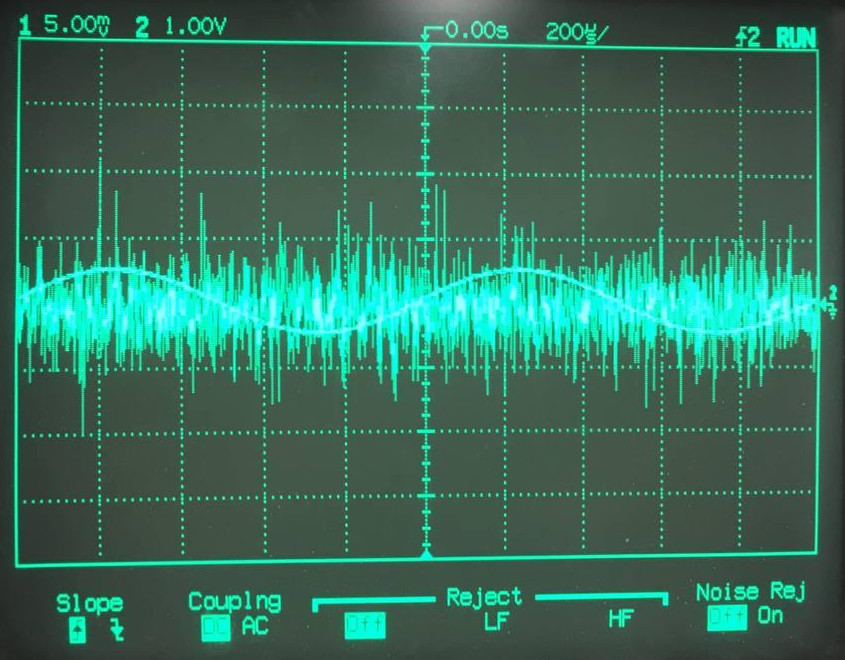
\includegraphics[scale = 0.5]{43c-SignalOszi.jpg}
    \captionof{figure}{Signal des Oszilloskops}
    \label{image:oszi}
    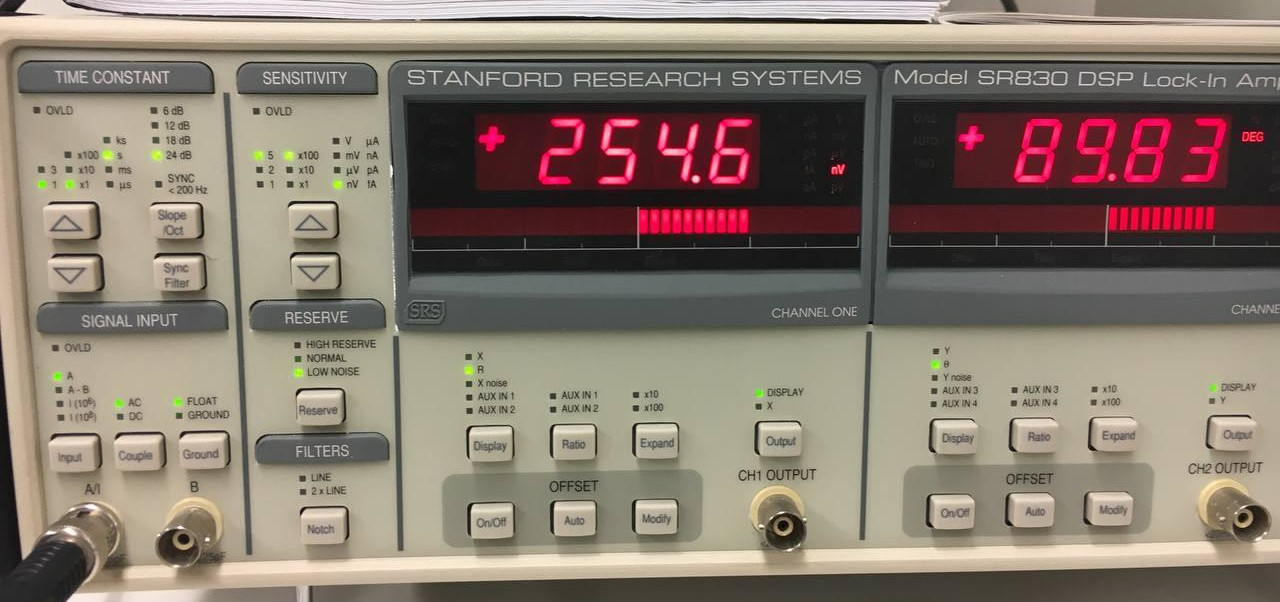
\includegraphics[scale = 0.4]{43c-EinstellungLockIn.jpg}
    \captionof{figure}{Einstellungen Lock-In-verstärker}
    \label{image:lockIn}
\end{center}
\section*{Aufzeichnungen während Versuch}
\begin{center}
    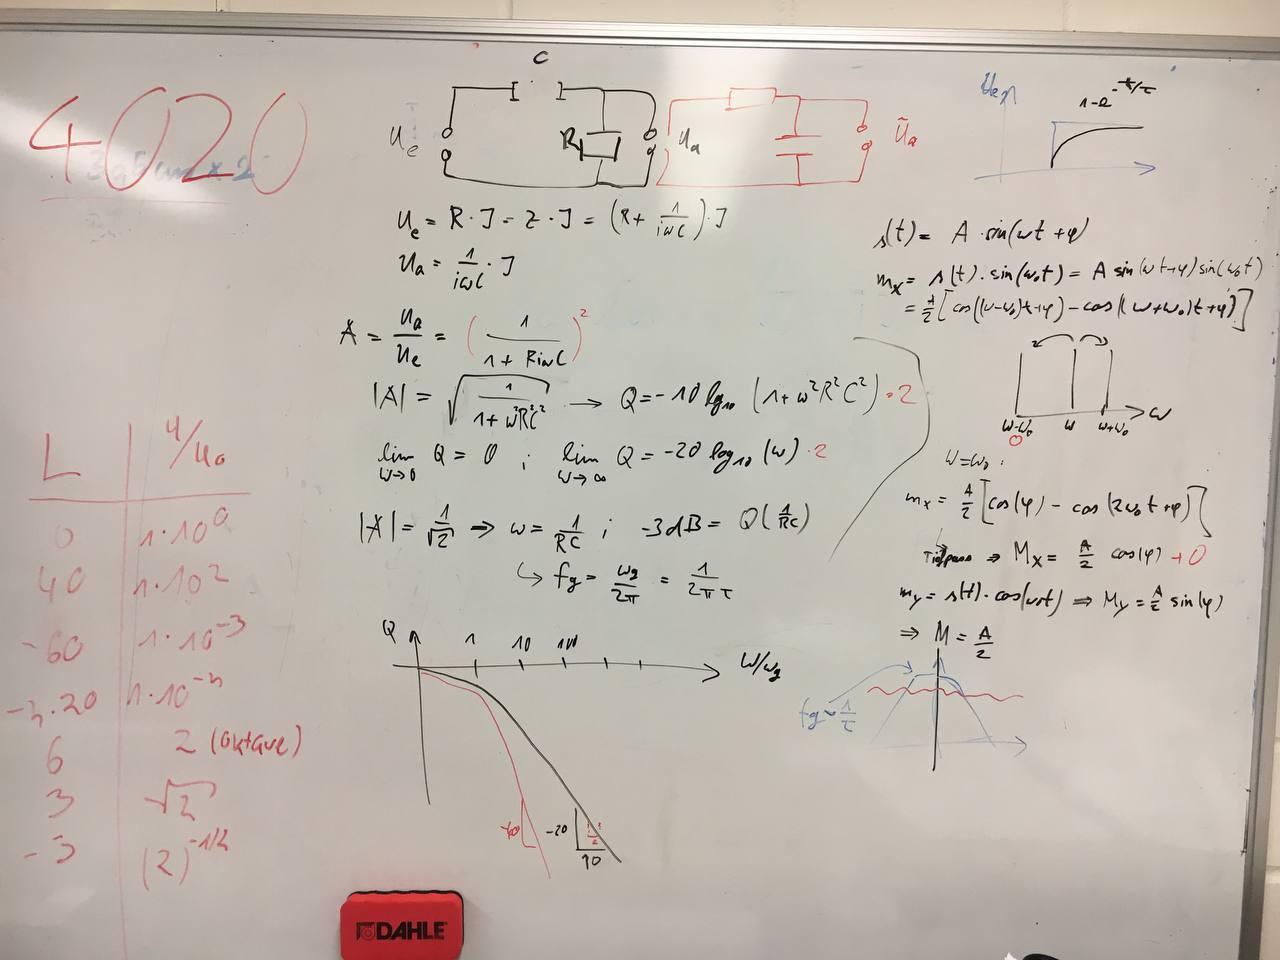
\includegraphics[scale = 0.4]{Aufzeichnungen.jpg}
    \captionof{figure}{Aufzeichnungen}
    \label{image:aufzeichnungen}
\end{center}
\newpage
\paragraph{b)}\textbf{Bandbreite Lock-In}\\
Sinusschwingung Amplitude = 100 mV\\
Schwankungen von $\pm\SI{0,0005}{\volt}$
\begin{center}
    \begin{tabular}{c c}
        $\tau$ = 30ms & \hspace{1cm} $\tau$ = 30ms\\
        Slope = 6dB & \hspace{1cm} Slope = 18dB\\
        \begin{tabular}{c | c}
            f/Hz & $U_{eff}$/V\\
            \hline
             700 & 0,0001 \\
             720 & 0,0001 \\
             740 & 0,0001 \\
             760 & 0,0001 \\
             780 & 0,0001 \\
             800 & 0,0017 \\
             820 & 0,0020 \\
             840 & 0,0020 \\
             860 & 0,0020 \\
             880 & 0,0030 \\
             900 & 0,0033 \\
             920 & 0,0040 \\
             940 & 0,0060 \\
             960 & 0,0090 \\
             980 & 0,0180 \\
            1000 & 0,0700 \\
            1020 & 0,0180 \\
            1040 & 0,0090 \\
            1060 & 0,0060 \\
            1080 & 0,0040 \\
            1100 & 0,0033 \\
            1120 & 0,0030 \\
            1140 & 0,0020 \\
            1160 & 0,0020 \\
            1180 & 0,0020 \\
            1200 & 0,0020 \\
            1220 & 0,0001 \\
            1240 & 0,0001 \\
            1260 & 0,0001 \\
            1280 & 0,0001 \\
            1300 & 0,0001 \\
        \end{tabular}
        & \hspace{1cm}
        \begin{tabular}{c | c}
            f/Hz & $U_{eff}$/V\\
            \hline
             950 & 0,0001 \\
             955 & 0,0001 \\
             960 & 0,0001 \\
             965 & 0,0002 \\
             970 & 0,0004 \\
             975 & 0,0006 \\
             980 & 0,0012 \\
             985 & 0,0026 \\
             990 & 0,0070 \\
             995 & 0,0270 \\
            1000 & 0,0706 \\
            1005 & 0,0270 \\
            1010 & 0,0073 \\
            1015 & 0,0026 \\
            1020 & 0,0012 \\
            1025 & 0,0006 \\
            1030 & 0,0004 \\
            1035 & 0,0002 \\
            1040 & 0,0001 \\
            1045 & 0,0001 \\
            1050 & 0,0001 \\
        \end{tabular}
    \end{tabular}
\end{center}
\newpage
\section*{Bestimmung Uhrzeit mit Oszilloskop}
Mit einem Kabel, welches aus dem Fenster um einen Baum gewickelt wurde und an das Oszilloskop angeschlossen ist, konnte auf dem Oszilloskop eine Art Morse-Signal empfangen werden. Dieses Signal nutzen Digitaluhren, um die Uhrzeit richtig zustellen.

\textbf{Signal:}\\
\textbf{. . - . - . . . . - 
        . - . - - . . - . . 
        - - . . . - . - - - 
        . . - - . - - . - . 
        . . . - . . . . . - 
        - . . . . - . . . }\\
\textbf{Decodierung:}\\
Zum Decodieren benutzen wir die Vorlage des Betreuers und beginnen mit dem 21. Stelle des Signals und erhalten: 51min 19h 5.Day 2.Weekday 10.Month 21.Year \\$\Rightarrow$ \textbf{Di 5.10.21 19:51}